\documentclass[useAMS,usenatbib]{mn2e}
\usepackage{footnote,graphicx,natbib,color,multirow,amsmath,url}
\voffset=-0.5in
\pdfminorversion=5
\setlength{\parsep}{0pt}
\setlength{\partopsep}{0pt}

\def\starpy ~{\textsc{starpy}}
\def\lesssim{\mathrel{\hbox{\rlap{\hbox{\lower3pt\hbox{$\sim$}}}\hbox{\raise2pt\hbox{$<$}}}}}
\font\nbf=cmssbx10 at 12.28pt %big font for headers


\begin{document}


\title[Group environment quenching mechanisms]{Galaxy Zoo: The interplay of quenching mechanisms in the group environment}
\author[Smethurst et al. 2015]{R. ~J. ~Smethurst,$^{1}$ C. ~J. ~Lintott,$^{1}$ and the Galaxy Zoo team \footnotemark[1]
\\ $^1$ Oxford Astrophysics, Department of Physics, University of Oxford, Denys Wilkinson Building, Keble Road, Oxford, OX1 3RH, UK 
}

\maketitle

\begin{abstract}
Does the environment of a galaxy directly influence the quenching history of a galaxy? Here we construct a sample of group and field galaxies with morphological classifications from Galaxy Zoo 2 and use Bayesian inference to determine the quenching time and exponential timescale that describes a simple SFH for a given galaxy from its photometry. We observe how the detailed morphological structures, such as bars and bulges, are affected by the group environment and correlate this with changes in the quenching history.  We find that the environment does play a direct role in galaxy quenching through a mechanism which is correlated to the halo mass of a group but not to the relative velocity of a satellite galaxy to its central. Environmental quenching mechanisms which are correlated with satellite velocity, such as ram pressure stripping, are not the main cause of quenching in the group environment. Instead an interplay of merger, mass, morphology and environmental quenching mechanisms dependant on the group potential drive the evolution of group galaxies. 

\end{abstract}

\begin{keywords}
galaxies -- environment, galaxies -- photometry, galaxies -- statistics, galaxies -- morphology
\end{keywords}

\footnotetext[1]{This investigation has been made possible by the participation of over 350,000 users in the Galaxy Zoo project. Their contributions are acknowledged at \url{http://authors.galaxyzoo.org}}

\section{Introduction}\label{sec:intro}
 
 There are many mechanisms which are proposed to cause quenching; including mergers \citep{daddi10, darg10b, cheung12, barro13, pontzen16}, AGN feedback \citep{dimatteo05, nandra07}, mass quenching \citep{peng12}, morphological quenching \citep{fang13} and the environment of a galaxy \citep[see review of mechanisms in][and references therein]{boselli06}.
 
 The galaxy environment as a cause of quenching was proposed due to the correlation of morphology \citep{dressler80, smail97, poggianti99, postman05, bamford09}, star formation rate (SFR) and the quenched galaxy fraction \citep{kauffmann03, baldry06, peng12, darvish16} with environmental density. However, do these correlations truly imply causation? Recent evidence from simulations suggests that the environment may not be the dominant quenching mechanism in the galaxy lifecycle. Perhaps instead, the correlation of increased galaxy quenched fractions with environment is due to a superposition of the effects of mergers \& interactions and both mass \& morphology quenching. 
 
\subsection{Mergers as a quenching mechanism}
In denser environments, galaxies are more likely to encounter another galaxy in a merger or interaction scenario than when isolated in the field environment. When two galaxies merge, the influx of cold gas funnelled by the forces in the interaction often result in energetic starbursts and the fuelling of a central AGN \citep{hopkins05}, both of which can exhaust  (and in the case of the AGN possibly expel) the gas required for star formation, effectively quenching the post-merger remnant galaxy \citep{pontzen16}. 

\subsection{Mass quenching}
Mass quenching is the process by which a galaxy, independent of its environment, uses up its available gas for star formation via the Kennicutt-Schmidt law \citep{schmidt59, kennicutt98} and consequently grows in mass. This is thought to be the dominant mechanism for isolated galaxies in the field \citep{kormendy04}. In groups and cluster environments, infall into the group can occur over long timescales during which gas reservoirs can be depleted via this mass quenching process.
 
\subsection{Morphological quenching}
Morphological quenching (or secular quenching) is the process by which the internal structure of a galaxy can impact on its SFR. This is theorised to occur in galaxies hosting bars; the bar funnels gas to the centre of the galaxy \citep{athanassoula92a} where it is exhausted by star formation effectively quenching the galaxy \citep{sheth05, zurita04, masters10c}. Such a process has been postulated to be caused also by bulges \citep{bluck14} and spiral \citep{hart16} structures in galaxies. 
  
\subsection{Environmental quenching}
The mechanisms under the umbrella of environmental quenching are  numerous and varied. Together with the typical gravitational galaxy-galaxy interactions \citep{moore96}, environmental quenching also encapsulates hydrodynamic interactions occurring between the cold inter stellar medium (ISM) of the in-falling galaxy and the hot intergalactic medium (IGM) of the group or cluster. This includes such processes as ram pressure stripping \citep{gunngott72}, viscous stripping \citep{nulsen82}, and thermal evaporation \citep[a rapid rise in temperature of the ISM due to contact with the IGM;][]{cowie77}. Starvation \citep{larson80} can remove the outer galaxy halo cutting off the star formation gas supply to a galaxy and preprocessing occurs when all of the above mechanisms take place in a group of galaxies which then falls into a larger cluster \citep{dressler04}. 

The most likely candidate (and therefore the most studied) mechanism for the cause of the environmental density-morphology and SFR relations is ram pressure stripping \citep[RPS;][]{abadi99, poggianti99}. However, there has been mounting evidence that RPS may not be effective at quenching as first thought \citep{emerick16, fillingham16}. 

\subsection{Aims of this work} 
In order to isolate the case of the density-morphology and density-SFR correlations, we need to study how galaxy quenching timescales and morphology change in group and field environments with different properties. We use the group environment to study this problem, as this is a more typical environment for a galaxy than the relatively rare rich cluster environment \citep{carlberg04}. To do this we construct a sample of both group and field galaxies and utilise Bayesian inference to determine the quenching time and exponential timescale to describe a simple SFH for a galaxy given its photometry. We aim to determine the following: (i) How does the environment influence the detailed morphological structures of a galaxy?  (ii) Is environmental quenching occurring in the group environment?

In Section~\ref{sec:data} we describe our data sources and inference methods and highlight our results in Section~\ref{sec:results}. We then discuss these results and how they fit into the bigger picture of quenching in Section~\ref{sec:disc}. The zero points of all magnitudes are in the AB system. Where necessary, we adopt the WMAP Seven-Year Cosmology \citep{jarosik11} with $(\Omega_m , ~\Omega_\Lambda , ~h) = (0.26, 0.73, 0.71)$.

 
\section{Data and Methods}\label{sec:data}

\subsection{Data Sources}\label{sec:photo}

\begin{figure*}
\centering{
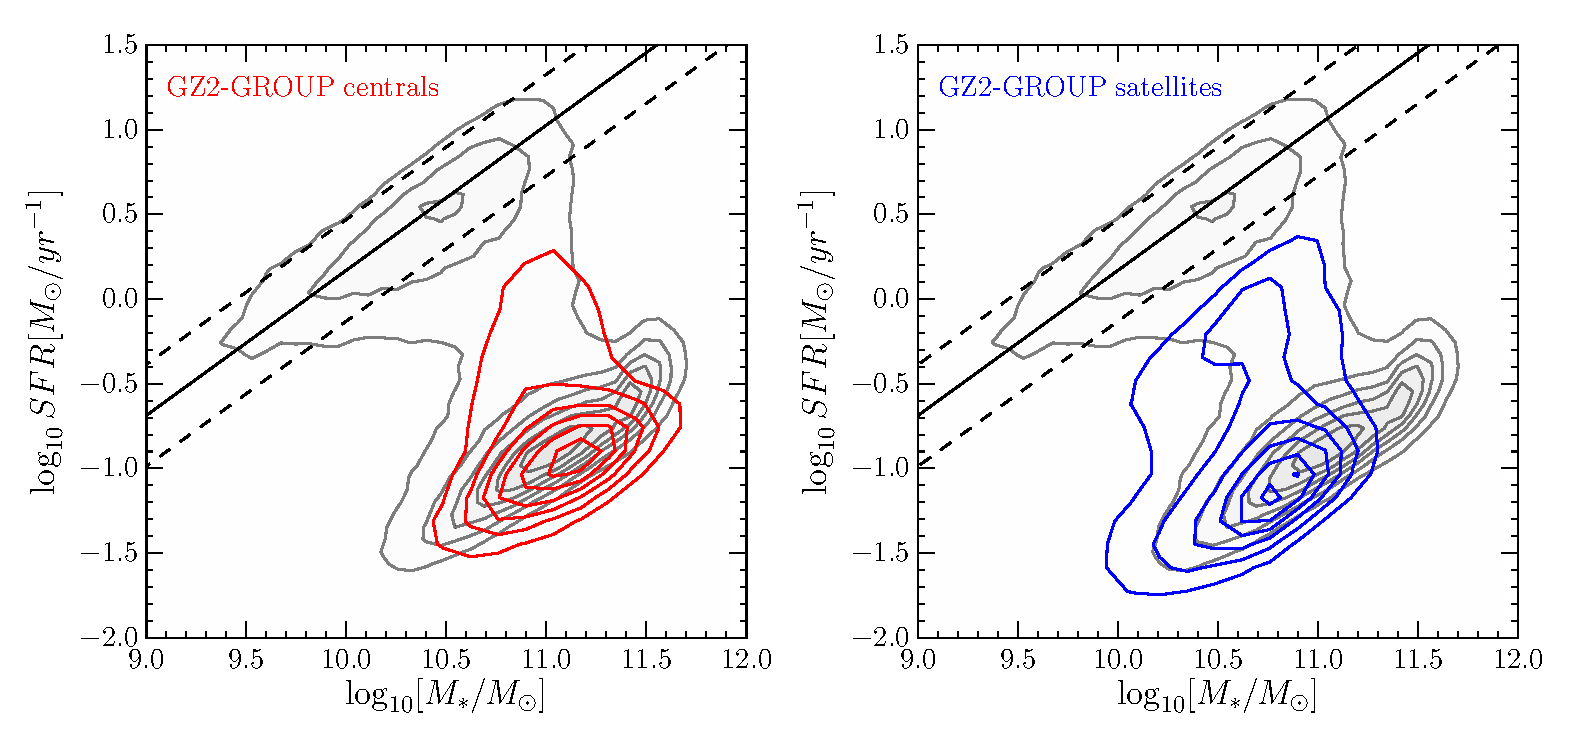
\includegraphics[width=0.95\textwidth]{sfr_mass_quenched_centrals_satellites_gz2_group.pdf}
\caption{The SFR-stellar mass plane showing central (left; red contours) and satellite (right; blue contours) galaxies in the \textsc{gz2-group} sample. In both panels the entire SDSS sample from the MPA-JHU catalog is shown by the grey filled contours. The definition of the star forming ``main sequence'' from \citet{Peng10} at $\overline{z}=0.083$ (solid line, the mean redshift of the \textsc{agn-host} sample) with $\pm 1\sigma$ (dashed lines) is shown.}}
\label{fig:sfrmass}
\end{figure*}

In this investigation we use visual classifications of galaxy morphologies from the Galaxy Zoo 2\footnote{\url{http://zoo2.galaxyzoo.org/}} (GZ2) citizen science project \citep{GZ2}, which obtains multiple independent classifications for each optical image. The full question tree for an image is shown in Figure~1 of \citeauthor{GZ2}  The GZ2 project used $304, 022$ images from the Sloan Digital Sky Survey Data Release 7 (SDSS; \citealt{york00, abazajian09}) all classified by \emph{at least} 17 independent users, with a mean number of classifications of $\sim42$.

Further to this, we required NUV photometry from the GALEX survey \citep{martin05}, within which $\sim42\%$ of the GZ2 sample was observed, giving $126, 316$ galaxies total ($0.01 < z < 0.25$). This will be referred to as the \textsc{gz2-galex} sample. The completeness of this sample ($-22 < M_u < -15$) is shown in Figure~2 of \cite{smethurst15}. 

Observed fluxes are corrected for galactic extinction \citep{Oh11} by applying the \citet{cardelli89} law. We also adopt $k$-corrections to $z = 0.0$ and obtain absolute magnitudes from the NYU-VAGC \citep{blanton05, blanton07, padmanabhan08}.


\subsubsection{Group Identification}\label{sec:groups}

We used the \citet{berlind06} catalogue, which uses a friends-of-friends algorithm to identify group and cluster galaxies in the SDSS. This was cross matched to the \textsc{gz2-galex} sample and limited to $z < 0.1$ to ensure GALEX completeness of the red sequence (see \citealt{wyder07, yesuf14}). Centrals were selected as the most massive galaxy in a group and all others were designated as satellites (masses were calculated using the absolute r-band magnitude and $u-r$ colour and the method of \citealt{baldry06}).  The projected cluster centric radius, $R$, of all satellite galaxies was calculated from the projected separations of a satellite from its central (converted to $\rm{kpc}$ from a consideration of the observed redshift of the central galaxy) which was then normalised by the $R_{200}$ of the group (the radius within which the mass overdensity is 200 times the critical density; see \citealt{finn05}), often used as a proxy for the virial radius of the group \citep{navarro95}. This resulted in a sample of $14,199$ group galaxies with $3,468$ centrals and $10,731$ satellites within a projected cluster centric radius range of $0 < R/R_{200} < 25$ and $z < 0.084$. 

In this work we focus on galaxies which are either quenching or quenched and are more than $\pm1\sigma$ below the star forming `main sequence'. This encompasses $4629$ satellite and $2314$ central galaxies and will be referred to as the \textsc{gz2-group} sample. These galaxies are highlighted in the panels of Figure \ref{fig:sfrmass} and can be seen to lie below the `main sequence' of star formation. 

We obtain masses and velocity dispersions of galaxies in the \textsc{gz2-group} sample from the MPA-JHU catalogue \citep{kauffmann03, brinchmann04}.

\subsubsection{Field sample}\label{sec:field}

For all galaxies in the \textsc{gz2-galex} sample, we calculated the smallest projected cluster centric radii, $R/R_{200}$, from each of the central galaxies in the  \citet{berlind06} catalog and selected candidate field galaxies as those with (i) $R/R_{200} > 25$ and (ii) $\log\Sigma < -0.8$ \citep[a measure of environmental density from][]{baldry06}. This sample of field galaxy candidates was then matched in redshift and stellar mass firstly to the central galaxies of the \textsc{gz2-group} sample to give $2,309$ field galaxies with $z < 0.084$ which will be referred to as the \textsc{gz2-cent-field} sample. In this work we focus on galaxies which are either quenching or quenched and are more than $\pm1\sigma$ below the star forming `main sequence'. This encompasses $1,596$ field galaxies with $z < 0.084$ which will be referred to as the \textsc{gz2-cent-field-q} sample and used as a control sample when investigating the trends with central galaxy properties of the inferred quenching parameters. 

The redshift distribution of the \textsc{gz2-cent-field-q} sample is shown in comparison to the distribution of central galaxies in the \textsc{gz-group} sample in Figure~\ref{fig:zcompare}. %SDSS images of a random selection of galaxies from the \textsc{gz2-group} and \textsc{gz2-cent-field-q} samples are shown ordered by their GZ2 debiased vote fraction in Figure~\ref{fig:mosaic}. %KS test between samples?

Secondly, the field galaxy candidates were then matched in redshift and stellar mass to the satellite galaxies of the \textsc{gz2-group} sample to give $6,849$ field galaxies with $z < 0.084$ which will be referred to as the \textsc{gz2-sat-field}. These galaxies in the \textsc{gz2-sat-field} sample will be used as a control when investigating the morphological trends of satellite galaxies with environment. Note that the sample is not restricted to being $\pm1\sigma$ below the star forming `main sequence' in this case. %KS test between samples?

We obtain masses, SFRs and velocity dispersions of galaxies for all of the field samples described above from the MPA-JHU catalogue \citep{kauffmann03, brinchmann04}.

%We also select all those galaxies in the satellite matched sample $\pm1\sigma$ below the star forming `main sequence', giving $1,043$ quenching or quenched field galaxies which will be referred to as the \textsc{gz2-sat-field-q} sample. These galaxies in the \textsc{gz2-sat-field-q} sample will be used as a control when investigating the trends with environment of the inferred quenching parameters. 

\begin{figure}
\centering{
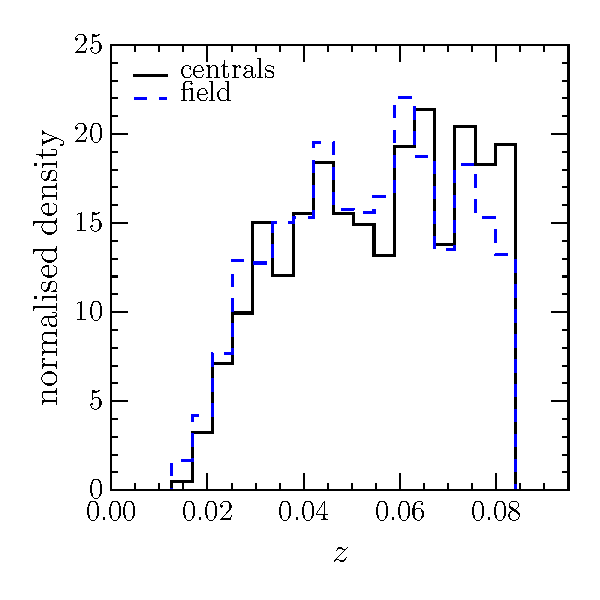
\includegraphics[width=0.45\textwidth]{redshift_cent_field.pdf}
\caption{Redshift distributions of central galaxies in the \textsc{gz2-group} sample (black solid line) in comparison to the redshift and mass matched \textsc{gz2-cent-field-q} sample (blue dashed line).}}
%KS Test between distributions?
\label{fig:zcompare}
\end{figure}
%
%\begin{figure*}
%\centering{
%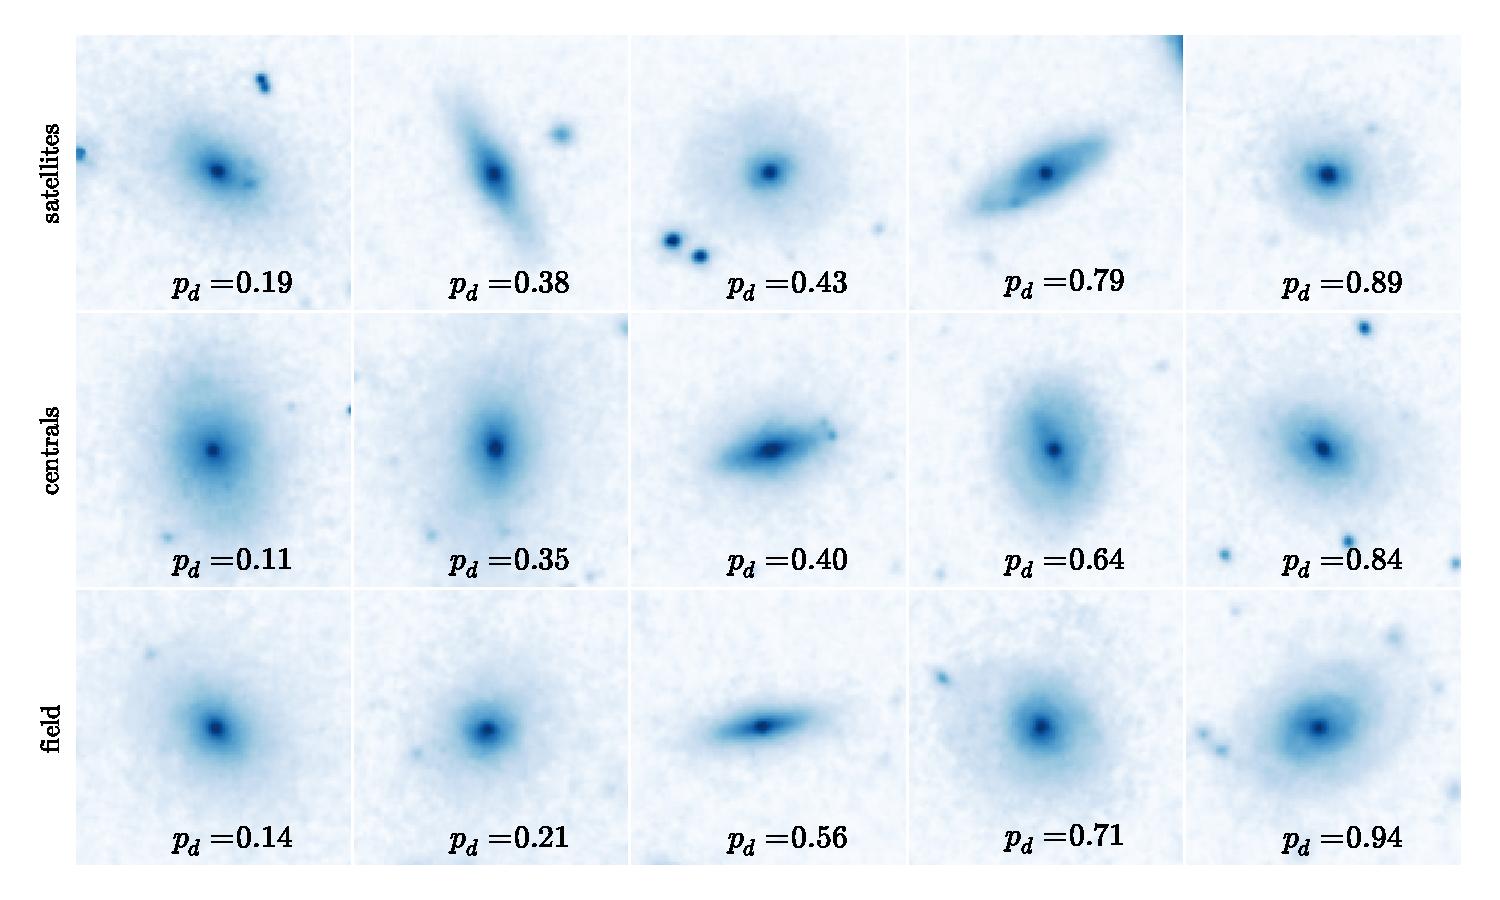
\includegraphics[width=0.95\textwidth]{mosaic_sat_cent_field_disc_fraction.pdf}
%\caption{Randomly selected SDSS \emph{gri} composite images of satellite and central galaxies in the \textsc{gz2-group} sample in comparison to those from the \textsc{gz2-field} sample. All galaxies lie within $0.04 < z < 0.05$ and in the central galaxy mass range $10^{10.5} < M_{*} [M_{\odot}] < 10^{11}$, used as a proxy for halo mass. The galaxies are ordered from least to most featured according to their debiased `disc or featured' vote fraction, $p_d$ (see \citealt{willett13}). The scale for each image is $0.099~\rm{arcsec/pixel}$.}}
%\label{fig:mosaic}
%\end{figure*}


\subsection{Deriving quenching parameters}\label{sec:starpy}

\textsc{starpy}\footnote{Publicly available: \url{http://github.com/zooniverse/starpy}} is a \textsc{python} code which allows the user to derive the quenching star formation history (SFH) of a single galaxy through a Bayesian Markov Chain Monte Carlo method \citep{emcee13}\footnote{\url{http://dan.iel.fm/emcee/}} with the input of the observed $u-r$ and $NUV-u$ colours, a redshift, and the use of the stellar population models of \cite{BC03}.  These models are implemented using solar metallicity (varying this does not substantially affect these results; \citealt{smethurst15}) and a Chabrier IMF \citep{chabrier03} but does not model for intrinsic dust. The SFH is modelled as an exponential decline of the SFR described by two parameters $[t_{q}, \tau]$, where $t_{q}$ is the time at the onset of quenching $\rm{[Gyr]}$ and $\tau$ is the exponential rate at which quenching occurs $\rm{[Gyr]}$. Under the simplifying assumption that all galaxies formed at $t=0$ $\rm{ Gyr}$ with an initial burst of star formation, the SFH can be described as: 
\begin{equation}\label{sfh}
SFR =
\begin{cases}
i_{sfr}(t_{q}) & \text{if } t < t_{q} \\
i_{sfr}(t_{q}) \times exp{\left( \frac{-(t-t_{q})}{\tau}\right)} & \text{if } t > t_{q} 
\end{cases}
\end{equation}
where $i_{sfr}$ is an initial constant star formation rate (SFR) dependent on $t_{q}$ \citep{schawinski14, smethurst15}.  A smaller $\tau$ value corresponds to a rapid quench, whereas a larger $\tau$ value corresponds to a slower quench. We note that a galaxy undergoing a slow quench is not necessarily quiescent by the time of observation. Similarly, despite a rapid quenching rate, star formation in a galaxy may still be ongoing at very low rates, rather than being fully quenched. This SFH model has previously been shown to appropriately characterise quenching galaxies \citep{Weiner06, Martin07, Noeske07,schawinski14}. We note also that star forming galaxies in this regime are fit by a constant SFR with a $t_{q} \simeq$ Age$(z)$, (i.e. the age of the Universe at the galaxy's observed redshift) with a very low probability.

The probabilistic fitting methods to these star formation histories for an observed galaxy are described in full detail in Section 3.2 of \cite{smethurst15}, wherein the \starpy ~~code was used to characterise the SFHs of each galaxy in the \textsc{gz2-galex} sample. We assume a flat prior on all the model parameters and the difference between the observed and predicted $u-r$ and $NUV-u$ colours are modelled as independent realisations of a double Gaussian likelihood function (Equation 2 in \citealt{smethurst15}). We also make the simplifying assumption that the age of each galaxy, $t_\mathrm{age}$ corresponds to the age of the Universe at its observed redshift, $t_\mathrm{obs}$.

We note also that galaxy colours were not corrected for intrinsic dust attenuation. This is of particular consequence for disc galaxies, where attenuation increases with increasing inclination. \cite{Buat05} found the median value of the attenuation in the GALEX NUV passband to be $\sim 1$ mag. Similarly \cite{masters10c} found a total extinction from face-on to edge-on spirals of 0.7 and 0.5 mag for the SDSS $u$ and $r$ passbands and show spirals with $\log(a/b) > 0.7$ have signs of significant dust attenuation. However, we showed from an investigation into this problem in Section~2.2 of \citet{smethurst16} that internal galactic extinction does not systematically bias our results from \starpy~. 

\begin{figure}
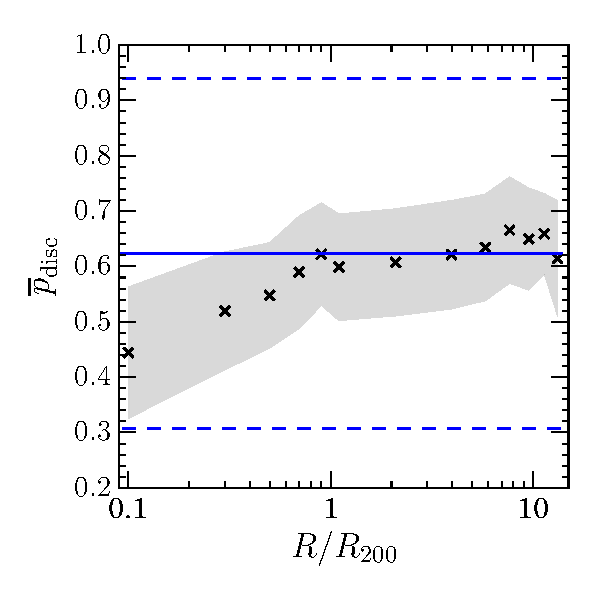
\includegraphics[width=0.46\textwidth]{p_disc_trend_with_log_radius_field_compare.pdf}
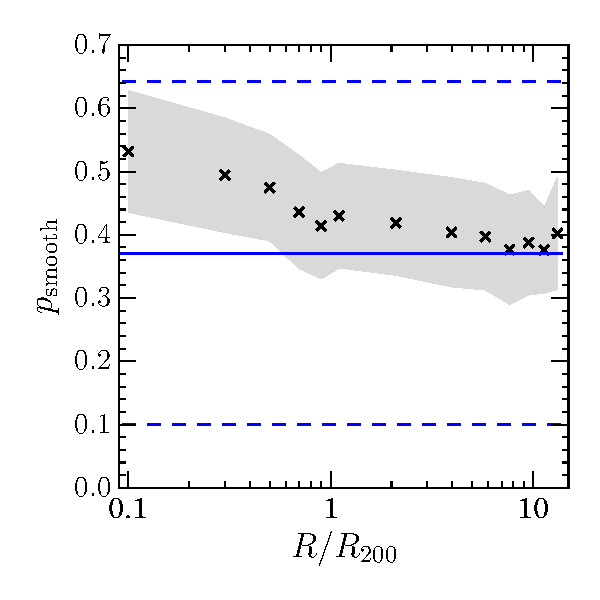
\includegraphics[width=0.46\textwidth]{p_smooth_trend_with_log_radius_field_compare.pdf}
\caption{Mean GZ vote fraction for disc (top) and smooth (bottom) galaxies in the \textsc{gz2-group} sample binned in projected cluster centric radius, normalised by $R_{200}$, a proxy for the virial radius of a group. The shaded region shows $\pm1\sigma$ on the mean vote fraction. The mean vote fraction of the \textsc{gz2-sat-field} sample are also shown (blue solid lines) with $\pm1\sigma$ (blue dashed lines).}
\label{fig:morphradius}
\end{figure}

\begin{figure}
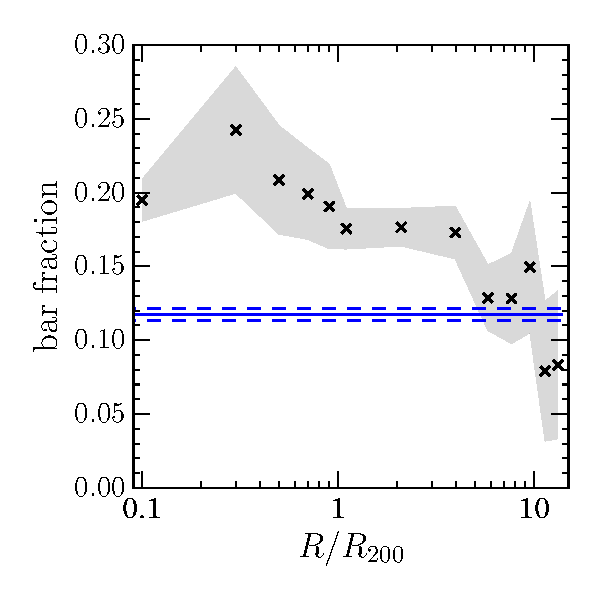
\includegraphics[width=0.46\textwidth]{bar_fraction_over_disc_trend_with_log_radius_sat_matched_field_cand.pdf}
\caption{Bar fraction (number of barred disc galaxies over number of disc galaxies) in the \textsc{gz2-group} sample binned in projected cluster centric radius, normalised by $R_{200}$, a proxy for the virial radius of a group. The shaded region shows $\pm1\sigma$ on the bar fraction. The bar fraction of the \textsc{gz2-sat-field} sample is also shown (blue solid line) with $\pm1\sigma$ (blue dashed line).}
\label{fig:barradius}
\end{figure}

\begin{figure}
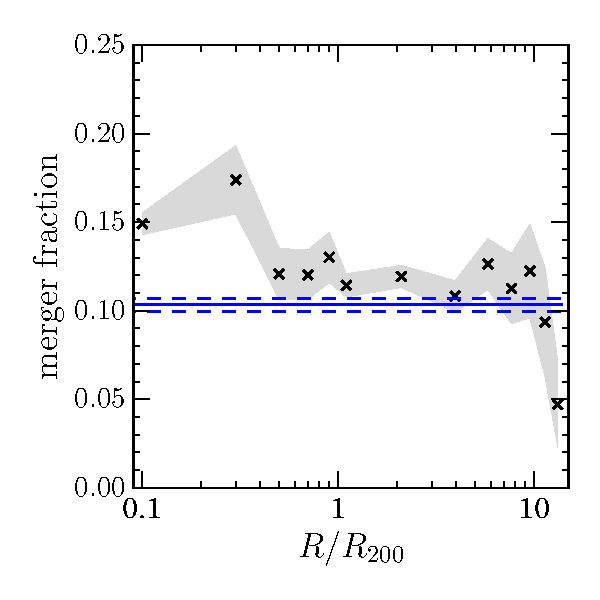
\includegraphics[width=0.46\textwidth]{merger_fraction_trend_with_log_radius_compare_sat_field_cand.pdf}
\caption{Merger fraction in the \textsc{gz2-group} sample binned in projected cluster centric radius, normalised by $R_{200}$, a proxy for the virial radius of a group. The shaded region shows $\pm1\sigma$ on the merger fraction. The merger fraction of the \textsc{gz2-sat-field} sample is also shown (blue solid line) with $\pm1\sigma$ (blue dashed line).}
\label{fig:mergerradius}
\end{figure}

The output of \starpy  ~ is probabilistic in nature and provides the posterior probability distribution across the two-parameter space for an individual galaxy the degeneracies for which can be seen in Figure~4 of \citet{smethurst15}.  Whereas in previous studies that distributions have been weight and combined to give an overall distribution representing the population of galaxies \citep[see][]{smethurst15, smethurst16}, due to the complex nature of the group environment here we choose instead to take the 50th percentile walker position of these individual posterior probability distributions to give the most likely $t_{q}$ and $\tau$ for each galaxy. \

This simplifies the output from \starpy  ~for each galaxy from a probability distribution to two more manageable values. In this work we will look for trends in the time since quenching onset, $\Delta t$, for a given galaxy by calculating {\bf $\Delta t = t_\mathrm{obs} - t_{q}$}. We will observe how this quantity changes with group properties, including halo mass (here we use the stellar mass of the group central as a proxy for halo mass), velocity dispersion, number of group members and relative velocity of a satellite galaxy. 

\section{Results}\label{sec:results}
\subsection{Dependence of detailed morphological structure with environment}

Figure \ref{fig:morphradius} shows the mean disc and smooth vote fractions from GZ2, binned in projected cluster centric radius (normalised by the approximate viral radius of each group, $R_{200}$). We can see that the mean disc (smooth) vote fraction decreases (increases) from the mean field value (blue line) under $1$ virial radius, in agreement with previous studies on the morphology-density relation \citep{dressler80, smail97, poggianti99, postman05, bamford09}. Along with this initial sanity check on the \textsc{gz2-group} sample, the extensive morphological classifications provided by GZ2 allows us to now investigate how more detailed morphological structure is affected by the group environment.  

Figure \ref{fig:barradius} shows how the bar fraction (number of barred disc galaxies over the number of disc galaxies) increases towards the centre of the group population, significantly over the field fraction (blue solid line). Figure \ref{fig:mergerradius} shows how the merger fraction does not significantly deviate from the field fraction (blue solid line) until within $\sim$ virial radius. Similarly, the left panel of Figure \ref{fig:bulgeradius} shows how those galaxies identified as having no or just noticeable bulges are less common in the inner regions of the cluster (left panel), whereas the fraction of galaxies with obvious or dominant bulges increases with decreasing projected distance from the centre of the cluster.

%Figure \ref{fig:sfrradius} shows how the SFR of the \textsc{gz2-group} sample does indeed decline with decreasing cluster centric distance, significantly below the mean SFR of the \textsc{gz2-field} sample shown by the blue dashed line. This is in agreement with the results of \cite{gomez03} who observe a similar decline in SFR with cluster centric radius in SDSS clusters (see for example, Figure 6 in \citealt{gomez03}). This coincides with the morphological fraction changes seen in Figures~\ref{fig:morphradius}-{\ref{fig:merger radius} in support of the conclusions of \citet{smethurst15} that quenching is morphologically dependant. 


%\begin{figure}
%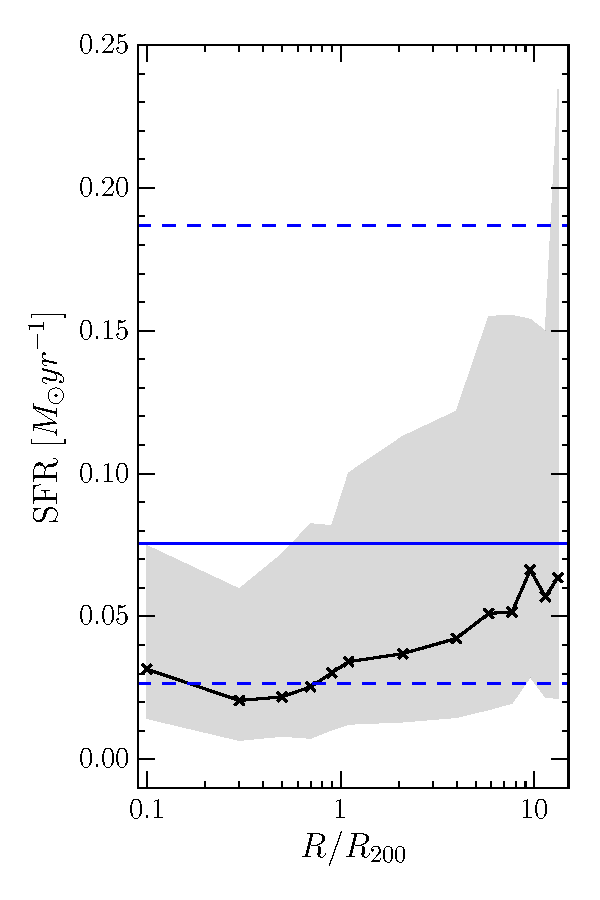
\includegraphics[width=0.46\textwidth]{sfr_trend_with_log_radius_field_matched_blue_dashed_hlines_gomez_03_rv_not_r200.pdf}
%\caption{Median $H\alpha$ derived star formation rates of satellite galaxies in the \textsc{gz2-group} sample, binned in projected cluster centric radius, normalised by $R_{200}$, a proxy for the virial radius of a group.  The shaded region shows the SFRs encompassed by $50\%$ of the population in a given bin. The median SFR of the \textsc{gz2-sat-field} sample is shown (blue solid line) along with the 25th and 75th percentiles (blue dashed lines).}
%\label{fig:sfrradius}
%\end{figure}

\subsection{Quenching times in the group environment}

\begin{figure*}
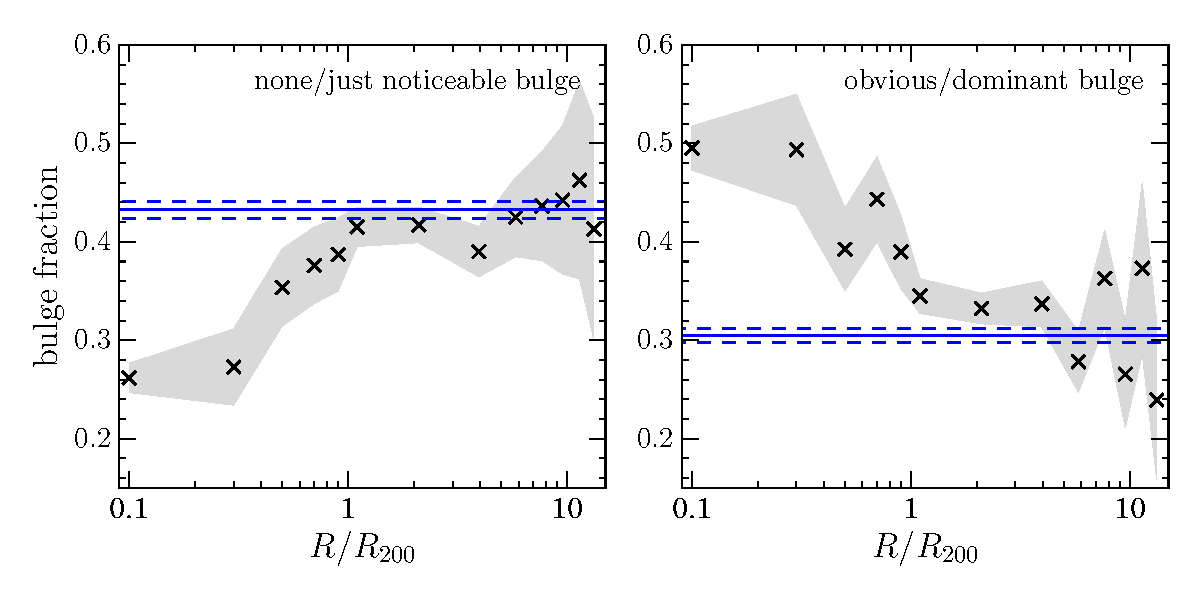
\includegraphics[width=0.85\textwidth]{min_max_bulge_fraction_trend_with_log_radius_sat_field_cand.pdf}
\caption{Fraction of galaxies with none/just noticeable bulge classifications (left) and with obvious/dominant bulge classifications (right) in the \textsc{gz2-group} sample binned in projected cluster centric radius, normalised by $R_{200}$, a proxy for the virial radius of a group. The shaded regions shows $\pm1\sigma$ on the bulge fractions. The bulge fractions of the \textsc{gz2-sat-field} sample are also shown (blue solid lines) with $\pm1\sigma$ (blue dashed lines).}
\label{fig:bulgeradius}
\end{figure*}

\begin{figure}
\centering{
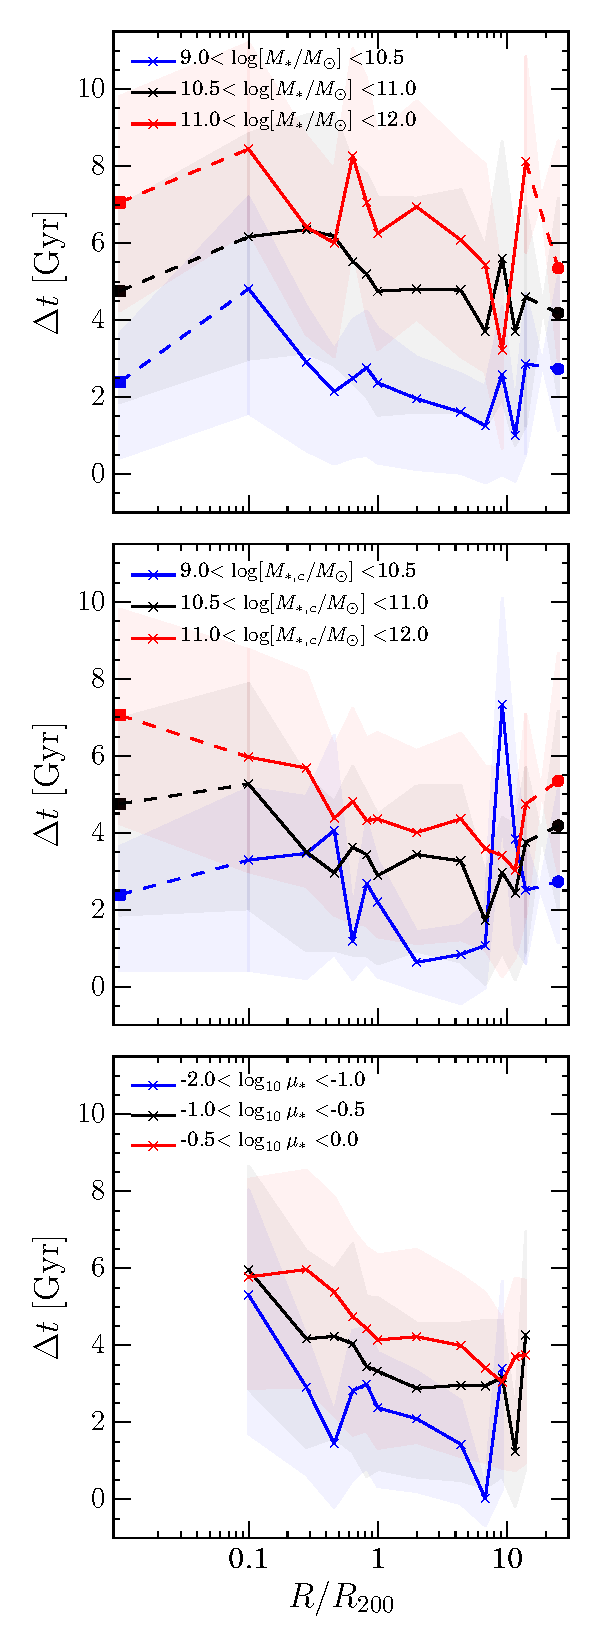
\includegraphics[height=0.85\textheight]{time_since_quenching_M*_Mh_mu.pdf}
\caption{The time since quenching onset ($\Delta t = t_{obs} - t_{q}$) binned in projected cluster centric radius, normalised by $R_{200}$, for satellite galaxies (crosses) split into bins of stellar mass (top), stellar mass of the corresponding central galaxy (middle; a proxy for halo mass of a group) and the stellar mass ratio ($\mu_* = M_*/M_{*,c}$, bottom). The corresponding values for central galaxies (squares, plotted at $0.01 R/R_{200}$) and galaxies in the \textsc{gz2-cent-field-q} sample (circles, plotted at $25 R/R_{200}$) are shown where calculable and connected by the dashed lines to help guide the eye. The shaded regions show the $\pm1\sigma$ on $\Delta t$ in each bin of $R/R_{200}$.}
\label{fig:timesinceradius}}
\end{figure}

\begin{figure}
\centering{
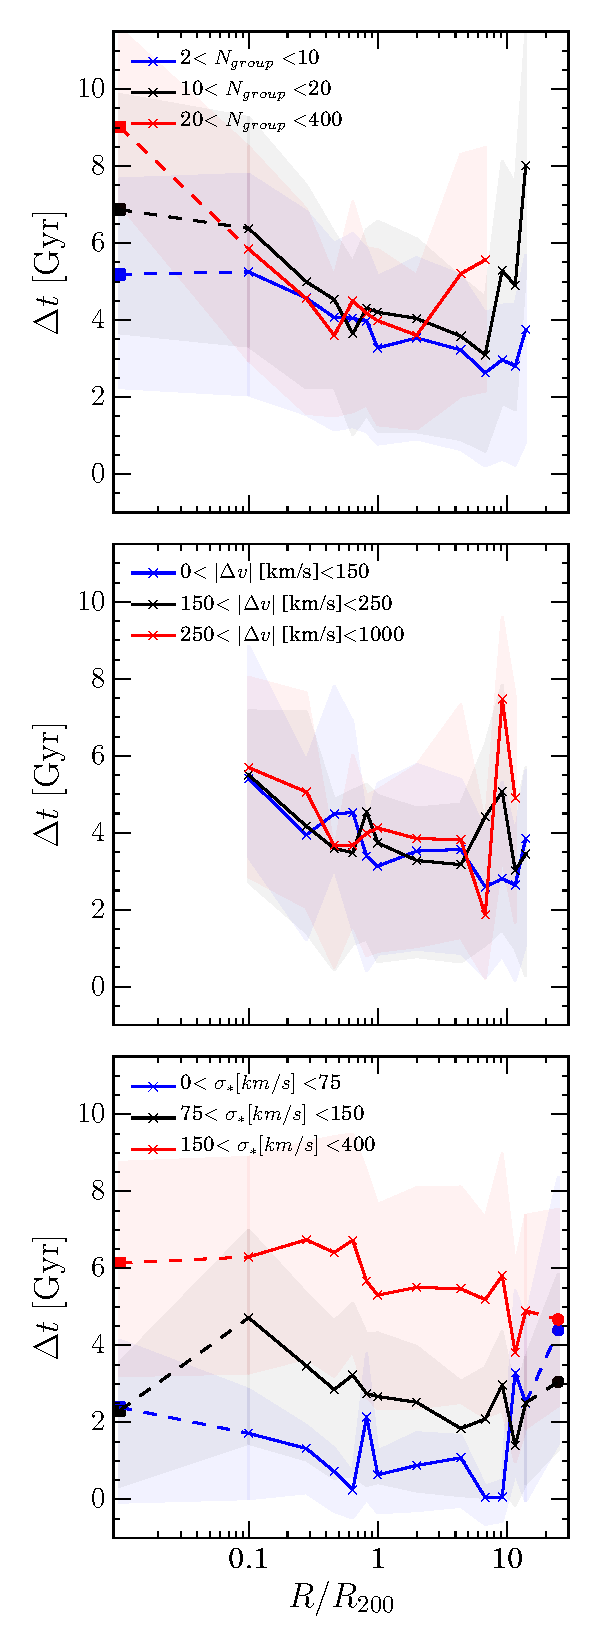
\includegraphics[height=0.85\textheight]{time_since_quenching_Ngroup_delv_sigma.pdf}
\caption{The time since quenching onset ($\Delta t = t_{obs} - t_{q}$) binned in projected cluster centric radius, normalised by $R_{200}$, for satellite galaxies (crosses) split by the number of group members ($N_{group}$, top), absolute relative velocity of the satellite to its central galaxy ($|\Delta v|$, middle) and velocity dispersion ($\sigma_*$, bottom). The corresponding values for central galaxies (squares, plotted at $0.01 R/R_{200}$) and galaxies in the \textsc{gz2-cent-field-q} sample (circles, plotted at $25 R/R_{200}$) are shown where calculable and connected to the satellite values by the dashed lines to help guide the eye. The shaded regions show the $\pm1\sigma$ on $\Delta t$ in each bin of $R/R_{200}$.}
\label{fig:timesinceradiusvel}}
\end{figure}


With the output from \starpy~ we can also study the time since quenching onset ($\Delta t = t_{obs} - t_{q}$, see Section \ref{sec:starpy}) binned in projected cluster centric radius, normalised by $R_{200}$ (a proxy for virial radius) for satellite galaxies and central galaxies in the \textsc{gz2-group} sample, compared with galaxies in the \textsc{gz2-field} sample. This is shown in Figures \ref{fig:timesinceradius} \& \ref{fig:timesinceradiusvel} and we investigate trends in $\Delta t$ by binning by various group properties:
\begin{itemize}

\item{Stellar mass, $M_*$: in the top panel of Figure \ref{fig:timesinceradius} galaxies in the \textsc{gz2-group} sample are now split by their stellar mass and we see a clear trend for increasing time since quenching onset with increasing stellar mass for satellite, central and field galaxies. The central galaxies (shown by the square points at $\sim 0.01 R/R_{200}$) appear to have quenched more recently than the inner satellites (at $\sim0.1R/R_{200}$) 
of the same mass.}

\item{Halo mass: in the middle panel of Figure \ref{fig:timesinceradius} we use a proxy for halo mass by splitting by the \textsc{gz2-group} sample by the stellar mass of the corresponding central galaxy of a group, $M_{c,*}$ and find a clear trend for increasing time since quenching onset with increasing stellar mass of the group central for satellite, central and field galaxies.}

\item{Mass ratio, $\mu_* = M_*/M_{*,c}$: the stellar mass ratio of the satellite to its central galaxy. In the bottom panel of Figure \ref{fig:timesinceradius} we show the time since quenching of the \textsc{gz2-group} split into bins of $\log_{10}\mu_*$. The change in $\Delta t $ with projected cluster centric radius occurs more steeply (particularly beyond $\sim$ a virial radius) for satellite galaxies with much smaller masses than their group central ($-2.0 < \log_{10}\mu_* < -1.0$, shown by the blue curve).}

\item{Number of group members, $N_{group}$: the top panel of Figure \ref{fig:timesinceradiusvel} shows that there is no trend with time since quenching onset with increasing $N_{group}$ for satellite galaxies. The central galaxies (shown by the square points at $\sim 0.01 R/R_{200}$) however, do show a trend for increasing time since quenching with $N_group$.}

\item{Relative velocity, $|\Delta v|$: in the bottom panel of Figure \ref{fig:timesinceradiusvel} we split the satellite galaxies of the \textsc{gz2-group} sample into bins of relative velocity to their central galaxies. We can see that there is no trend with time since onset of quenching with increasing relative velocity for galaxies in the group environment.}

\item{Stellar velocity dispersion, $\sigma_*$: the bottom panel of Figure \ref{fig:timesinceradiusvel} shows the time since quenching of the \textsc{gz2-group} sample split into bins of $\sigma_*$. The stellar velocity dispersion shows the largest trend in $\Delta t$ for satellite galaxies of all of the group properties studied, with galaxies with the smallest (largest) stellar velocity dispersions have quenched more (less) recently. }
\end{itemize}

Across all the panels in Figures \ref{fig:timesinceradius} \& \ref{fig:timesinceradiusvel} we see a general trend for increasing time since quenching onset with decreasing distance from the group centre. As earlier, in Figures \ref{fig:morphradius}$-$\ref{fig:bulgeradius} significant differences from the field value arise inside $\sim$ one virial radius. 


\section{Discussion}\label{sec:disc}

\subsection{The role of mergers in quenching in the group environment}\label{sec:rolemergerenv}

The merger classification in GZ2 has been shown to preferentially identify major mergers \citep{darg10a}. Similarly, bulge formation in disc galaxies is often associated with (minor) merger driven evolutionary histories \citep{croton06, tonini16}.  Although we see evidence for an enhanced merger fraction in the inner regions of the group environment in Figure~\ref{fig:mergerradius}, the bulge fractions in Figure ~\ref{fig:bulgeradius} vary much more significantly from the field value than the merger fraction. This suggests that minor mergers may be more dominant than major mergers in the group environment, particularly at $R/R_{200} > 0.5$. 

If mergers are an important evolutionary mechanism for satellite galaxies, as the morphological evidence in Figures~\ref{fig:mergerradius} \& \ref{fig:bulgeradius} suggests, we would expect to see a difference in the quenching histories of satellites residing in groups with a larger number of members. However, the top panel of Figure \ref{fig:timesinceradiusvel} shows there is no trend with time since quenching onset with increasing $N_{group}$ for the satellite galaxies. This suggests that mergers are not the dominant quenching mechanism for satellite galaxies.

For central galaxies however, this is not the case. The central galaxies (shown by the square points at $\sim 0.01 R/R_{200}$ in the top panel of Figure \ref{fig:timesinceradiusvel}, do show a trend for increasing time since quenching with increasing $N_{group}$. Therefore, we can postulate that the larger the number of group members, the more important mergers are for a central's evolutionary history. 

This idea is supported by the result shown in the top panel of Figure~\ref{fig:timesinceradius} when the \textsc{gz2-group} is split into bins of stellar mass. We can see that centrals of a given mass have quenched more recently than the inner satellites (at $\sim0.1R/R_{200}$) of a given mass. This suggests that an episode of more recent star formation may have occurred in the central galaxies but not in the inner satellites. This is once again suggestive of a merger dominated evolutionary history for central galaxies, as mergers are thought to cause an energetic burst of star formation which in turn quenches the remnant galaxy \citep{hopkins05, treister12, pontzen16}. 


\subsection{The role of mass quenching in the group environment}\label{sec:rolemassenv}

The role of mass quenching in the group environment is apparent in the top panel of Figure~\ref{fig:timesinceradius} and the bottom panel of Figure~\ref{fig:timesinceradiusvel} where the \textsc{gz2-group} satellites are binned by stellar mass and central velocity dispersions respectively. We see a trend for increasing time since quenching with increasing stellar mass and velocity dispersion for centrals, satellites and field galaxies. This is suggestive of mass quenching occurring across the entire galaxy population irrespective of environmental density, supporting the work of \citet{peng10, gabor10, peng12, darvish16}

\subsection{The role of morphological quenching in the group environment}\label{sec:rolemorphenv}

The results in Figure \ref{fig:barradius}, showing the increasing bar fraction towards the central group regions which is consistent with results that show that bars themselves may be the cause of morphological quenching through the funnelling of gas toward the central regions of galaxies \citep{athanassoula92b, sheth05,masters10c}. However we must consider whether the environment itself may play a role in triggering the disk instabilities which can produce a morphological bar. Indeed harassment and tidal interactions have been shown to both promote and inhibit bar formation dependent on the stellar mass \citep{noguchi88, moore96, skibba12}.  In this case, morphological quenching would be occurring but indirectly due to environmental quenching. 

\subsection{The role of the environment in quenching}\label{sec:roleenv}

Across all panels of Figures ~\ref{fig:timesinceradius}-\ref{fig:timesinceradiusvel} a trend for increasing time since quenching onset with decreasing projected cluster centric radius is present. This suggests that the environment does directly cause quenching throughout the infall time of a galaxy in a group. Those galaxies closer in, fell into the group earlier and as they did so they started to quench, giving rise to a larger inferred $\Delta t$.

In the top panel of Figure \ref{fig:timesinceradius} we also see a clear trend for increasing $\Delta t$ with increasing stellar mass of the group central for both satellite and central galaxies. More massive halos therefore have a greater impact on the star formation histories of their satellites than less massive halos.  If we account for both the stellar mass and the halo mass of the central galaxy simultaneously by considering the stellar mass ratio of the satellite to its central galaxy, $\mu_* = M_*/M_{*,c}$ (see the bottom panel of Figure \ref{fig:timesinceradius}) we see that the change in $\Delta t $ with projected cluster centric radius occurs more steeply (particularly at $R/R_{200} \lesssim 1$) for satellite galaxies with much smaller masses than their group central. The stellar mass of the central galaxy is used as a proxy for halo mass which is correlated with both (i) the gravitational potential of the group and (ii) the temperature of the IGM.

This is thought that higher mass halos have hotter inter galactic medium (IGM) temperatures which can then have a greater impact impact on a galaxy through RPS of cold gas. If RPS is indeed a dominant environmental quenching mechanism we should see a trend in $\Delta t$ with the speed of a satellite galaxy relative to the group central.  However in the middle panel of Figure \ref{fig:timesinceradiusvel} we see that this is not the case. 

This suggests that any environmental quenching mechanism responsible for the trends seen in $\Delta t$ with the mass of the corresponding central galaxy and mass ratio of the satellite to its central (middle and bottom panels of Figure~\ref{fig:timesinceradius} respectively) are not corrected with satellite velocity. This therefore rules out RPS as the dominant environmental quenching mechanism, in support of the conclusions of \citet{emerick16, fillingham16}.  The dominant environmental quenching mechanism in the group environment must therefore be correlated with the group potential. This suggests that satellite galaxies may be most affected by gravitationally driven environmental effects, such as harassment and galaxy-galaxy interactions or by thermal evaporation of the galaxy halo due to the hot IGM. 

\subsection{The Big Picture}\label{sec:bigpic}

In the previous sections we have discussed how our results of the changing morphological features and quenching times with projected cluster centric radius in the group and field environments show evidence for both merger, mass, morphological and environmentally driven evolutionary histories. This suggests that not one mechanism is dominant in the group environment but that a superposition of all these effects gives rise to the observed morphology-density and morphology-SFR relations.

Just as galaxy morphology is a spectrum from disc-dominated to spheroid-dominated systems, so too are the quenching mechanisms which cause this morphological transformation. Mergers and interactions are a spectrum of mass ratios from micro mergers \citep{carlin16} through to major mergers, which have increasingly devastating impact upon the morphology and SFR of a galaxy. Morphological quenching mechanisms lie on a spectrum of stellar mass, having a larger impact on those galaxies with smaller masses. Environmental quenching mechanisms lie on a spectrum of increasing group potential, giving rise to a stronger impact on the SFR of smaller mass galaxies in larger halos.  

All of these mechanisms discussed are striving towards the same end result with no single mechanism dominating over the other, except in the most extreme of environments. Mechanisms traditionally associated with the field, such as mass \& morphology quenching also occur in more dense environments, however will often (after a long infall to the central regions of a group) be overwhelmed by those more rapid and violent mechanisms of mergers and interactions (and the triggered outflows from AGN that are associated with such mechanisms; see \citealt{smethurst16}). Similarly, environmental quenching mechanisms caused by the dense halo and hot IGM are influential as soon as a galaxy falls into a group or cluster, but such processes can also be interrupted momentarily by an interaction or a merger as a galaxy traverses the more dense environment.   


\section{Conclusions}\label{sec:conc}

Mergers, mass quenching morphology quenching and environmental quenching are all prevalent in galaxy groups. The environment does play a role in quenching galaxies through a mechanism proportional to the halo mass of the group but not proportional to the relative speed of the satellite galaxy to its central galaxy. This suggests that ram pressure stripping is not the dominant environmental quenching mechanism. All of these mechanisms discussed coalesce to give rise to the distributions in galaxy properties we see across the Universe through their constant interplay across cosmic time. 

\section*{Acknowledgements}

RS acknowledges funding from the Science and Technology Facilities Council Grant Code ST/K502236/1. 

The development of Galaxy Zoo was supported in part by the Alfred P. Sloan Foundation. Galaxy Zoo was supported by The Leverhulme Trust. 

Based on observations made with the NASA Galaxy Evolution Explorer.  GALEX is operated for NASA by the California Institute of Technology under NASA contract NAS5-98034

Funding for the SDSS and SDSS-II has been provided by the Alfred P. Sloan Foundation, the Participating Institutions, the National Science Foundation, the U.S. Department of Energy, the National Aeronautics and Space Administration, the Japanese Monbukagakusho, the Max Planck Society, and the Higher Education Funding Council for England. The SDSS Web Site is \url{http://www.sdss.org/}.
The SDSS is managed by the Astrophysical Research Consortium for the Participating Institutions. The Participating Institutions are the American Museum of Natural History, Astrophysical Institute Potsdam, University of Basel, University of Cambridge, Case Western Reserve University, University of Chicago, Drexel University, Fermilab, the Institute for Advanced Study, the Japan Participation Group, Johns Hopkins University, the Joint Institute for Nuclear Astrophysics, the Kavli Institute for Particle Astrophysics and Cosmology, the Korean Scientist Group, the Chinese Academy of Sciences (LAMOST), Los Alamos National Laboratory, the Max-Planck-Institute for Astronomy (MPIA), the Max-Planck-Institute for Astrophysics (MPA), New Mexico State University, Ohio State University, University of Pittsburgh, University of Portsmouth, Princeton University, the United States Naval Observatory, and the University of Washington.

This publication made extensive use of the Tool for Operations on Catalogues And Tables (TOPCAT; ~\citealt{taylor05}) which can be found at \url{http://www.star.bris.ac.uk/~mbt/topcat/} and the open source Python module \emph{astroPy}\footnote{\url{http://www.astropy.org/}}; \citealt{astropy13}). This research has also made use of NASA's ADS service and Cornell's ArXiv. 

\bibliographystyle{mn2e}
\bibliography{refs}  

\end{document}